\chapter{Load Testing}
We used Tsung~\cite{tsung} framework for load testing. We designed a \textit{generic workflow} which was able to capture the usual activities of a user while covering most, if not all, features of our website. We ran most of our tests on this generic workflow. Testing on the generic workflow gave us a rough idea on the overall performance of our website and possible bottlenecks. Later we created \textit{specific workflow} separating out the portions that we thought might be causing the greatest bottlenecks. We ran our tests on this specific workflow before and after optimization to verify that this was indeed the workflow that was causing the bottlenecks and that these have been remediated by the optimizations. Unless otherwise specified, all the tests documented in this report were run on a C5 large app server and a m4 large database server. The optimizations described in this section are incremental, that is, stacked over the previous optimization.

\section{Generic Workflow}\label{sec:generic-workflow}
In this workflow, at first a user logs in to the website. The user waits for a time between zero and two seconds, visits the games index page, and then waits again for a time between zero and one second. Then the user randomly visits a game page, waits for a time between zero and two seconds, comments on that game and then logs out. This concludes the first sessions of our workflow. 

In the second session, a user browses to the search page, searches for games by name, waits for a time between zero and one second, visits a random games page, waits for a time between zero and two seconds, searches for games by number of backgrounds, waits for a time between zero and two seconds, and visits a random game page. 

In the third session, a user browses to the gamers index page, waits between zero and one second, randomly gets a game, waits between zero and one second, browses to the genres page, waits between zero and one second, and finally browses to the companies page.

In the fourth session, a user browses to the signup page, waits for zero to three seconds, submits the form, waits for zero to one second, visits the games index page, waits for zero to one second, and finally likes/dislikes a random game.

For this workflow we had four arrival phases, the arrival rate being doubled at each consecutive phase and the very first one having an arrival rate of two users per second. Figure~\ref{fig:generic1} and ~\ref{fig:generic2} illustrate all the four sessions with the help of toned down sequence diagrams.

\begin{figure}
\subfloat[First session.]{%
  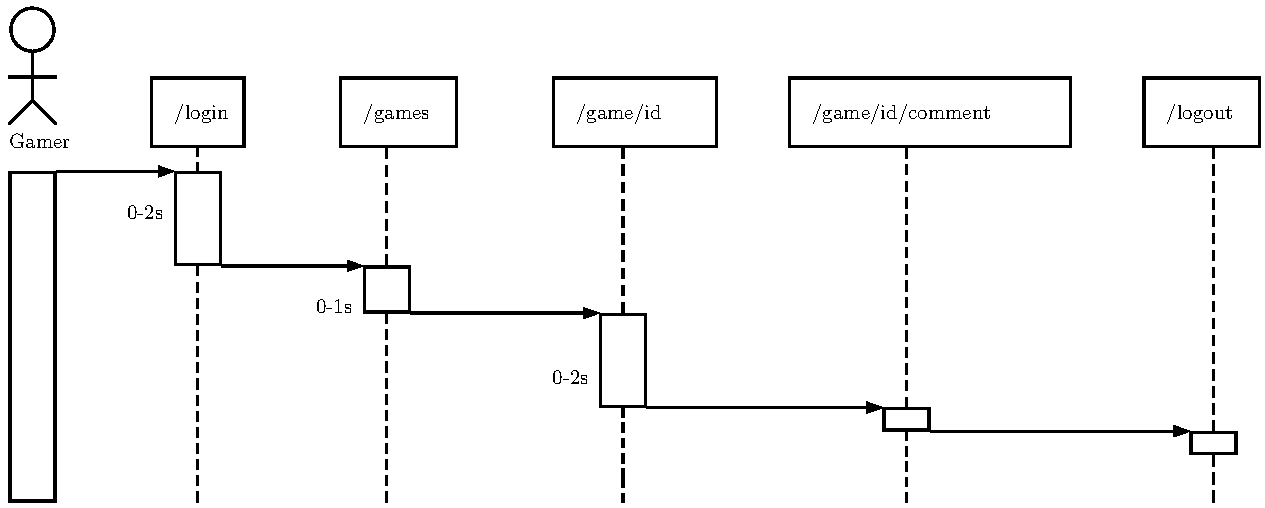
\includegraphics[clip,width=\columnwidth]{images/generic-1}%
}

\subfloat[Second session.]{%
  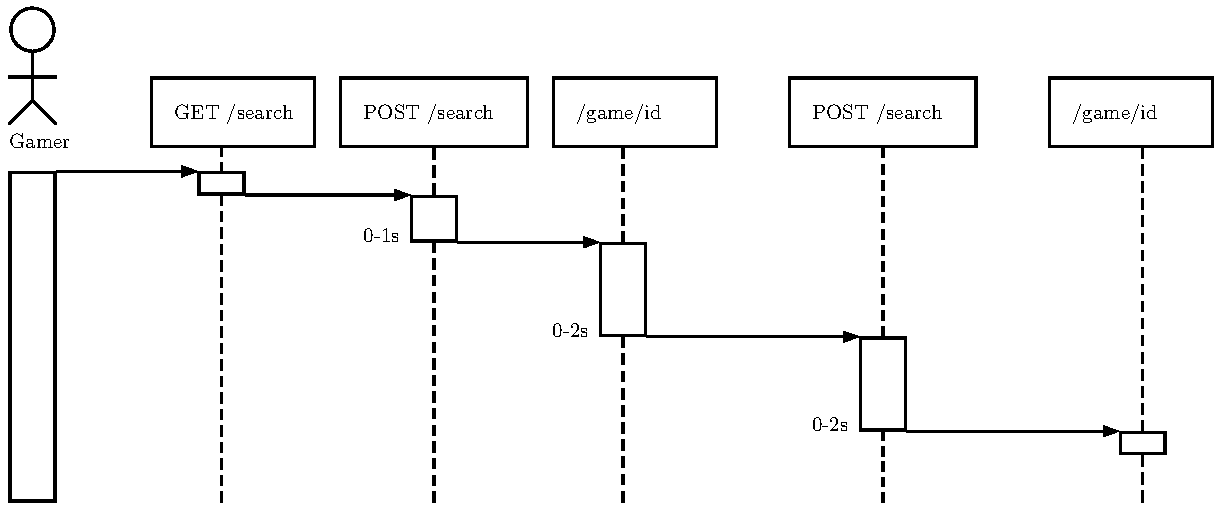
\includegraphics[clip,width=\columnwidth]{images/generic-2}%
}
\caption{First and second sessions of generic workflow.}\label{fig:generic1}
\end{figure}

\begin{figure}
\subfloat[Third session.]{%
  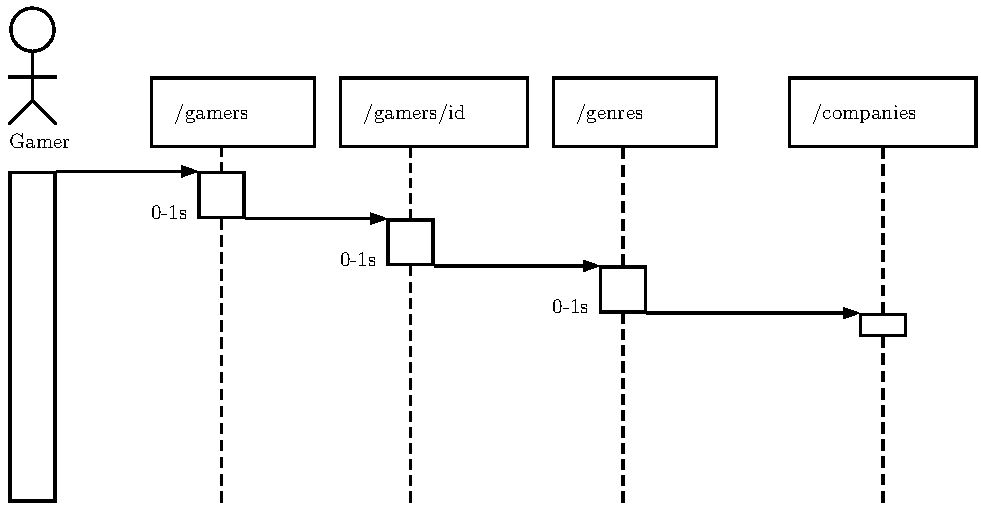
\includegraphics[clip,width=\columnwidth]{images/generic-3}%
}

\subfloat[Fourth session.]{%
  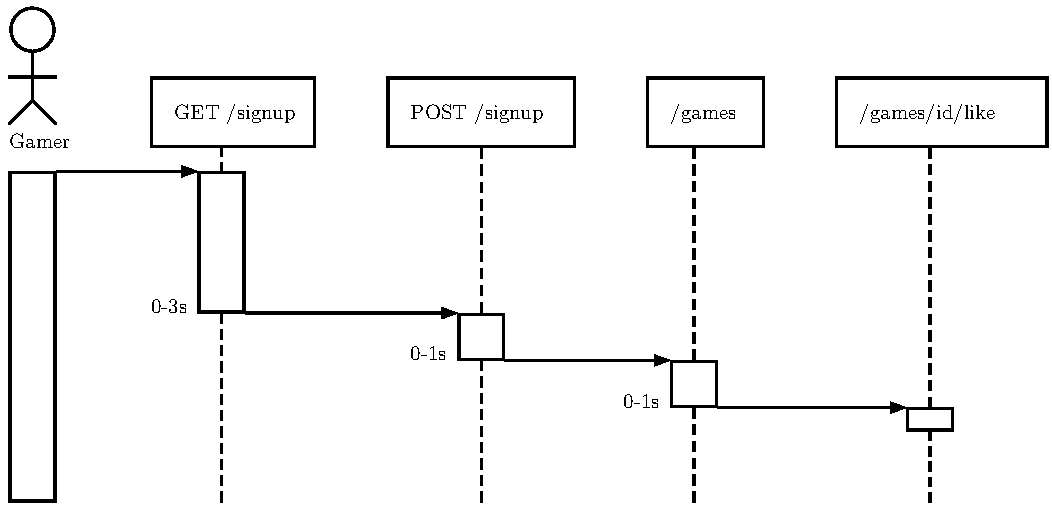
\includegraphics[clip,width=\columnwidth]{images/generic-4}%
}
\caption{Third and fourth sessions of generic workflow.}\label{fig:generic2}
\end{figure}

\section{Specific Workflow}\label{sec:specific-workflow}
It came to our observation that the number of sql queries being invoked in a couple of pages (index page of genres and companies) was higher than normal. We hypothesized optimizing the query in some way might improve our response time. Just to verify our hunch, we came up with a specific workflow and tested that before and after optimization. The exact optimization has been discussed in a later section.

In this workflow, a user hits the index page for games, followed by the index pages of genres and companies. For this workflow we had four arrival phases, the arrival rate being doubled at each consecutive phase and the very first one having an arrival rate of two users per second. Figure~\ref{fig:specific} illustrates the specific workflow with the help of a toned down sequence diagram.

\begin{figure}
	\centering
	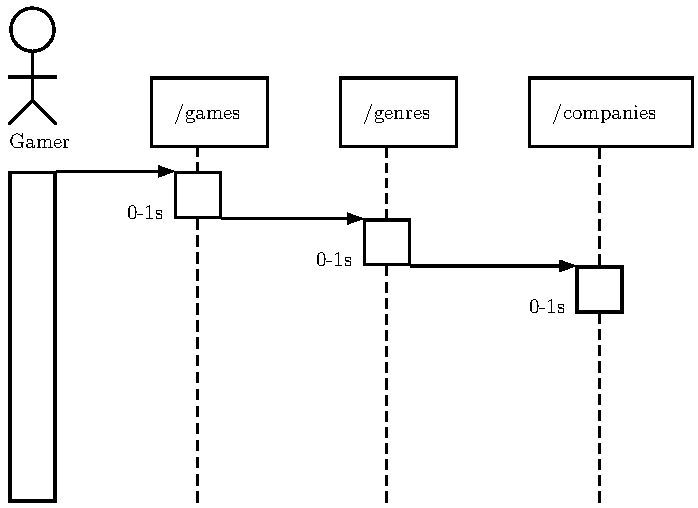
\includegraphics{images/specific}
	\caption{Specific workflow.}\label{fig:specific}
\end{figure}

\section{Optimization: AJAX}
We observed a huge number of 5xx response codes the first time our application was tested using the generic workflow. A quick look at the rails log revealed that for every game showed in the index page, a query was executed to get its likes/dislikes. Instead of showing this information automatically, we decided to invoke an AJAX request on hover over ``stats'' text. It was observed that this increased the number of 200 codes and decreaed the number of 5xx codes. Figure~\ref{fig:numcodes} shows the total number of 200 and 5xx codes over time for deployment without and with AJAX.
\begin{figure}
	\centering
	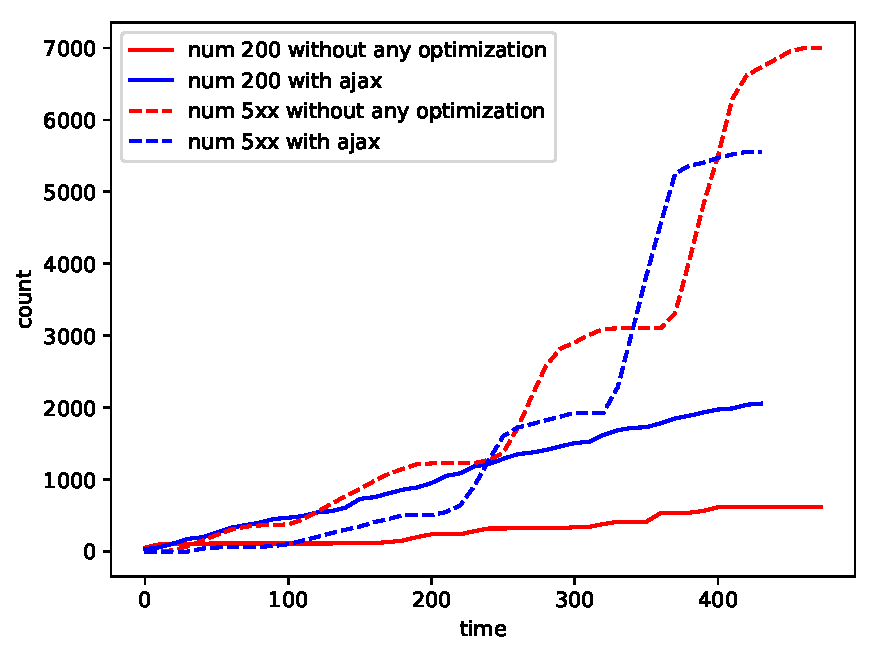
\includegraphics[width=0.8\textwidth]{images/without-any-optimization-with-ajax.pdf}
	\caption{HTTP response counts with and without ajax.}\label{fig:numcodes}
\end{figure}

\section{Optimization: Pagination}
Although the introduction of AJAX improved performance to some extent, the number of 5xx was still high. As the next step to optimization, we implemented pagination on the index page of games and comments page of individual games. Later on we implemented pagination on a few search pages too. Pagination increased the number of 200 codes further along with decreasing the number of 5xx codes. Figure~\ref{fig:aap} presents a graph of number of response codes along with a graph of mean duration of requests. It is evident that the introduction of pagination decreased the mean duration of requests. It is worth noting that in case of pagination the requests are serviced much faster, as a result of which it seems like there is a phase difference in the second graph and it completes much earlier.

\begin{figure}%
    \centering
    \subfloat[HTTP codes.]{{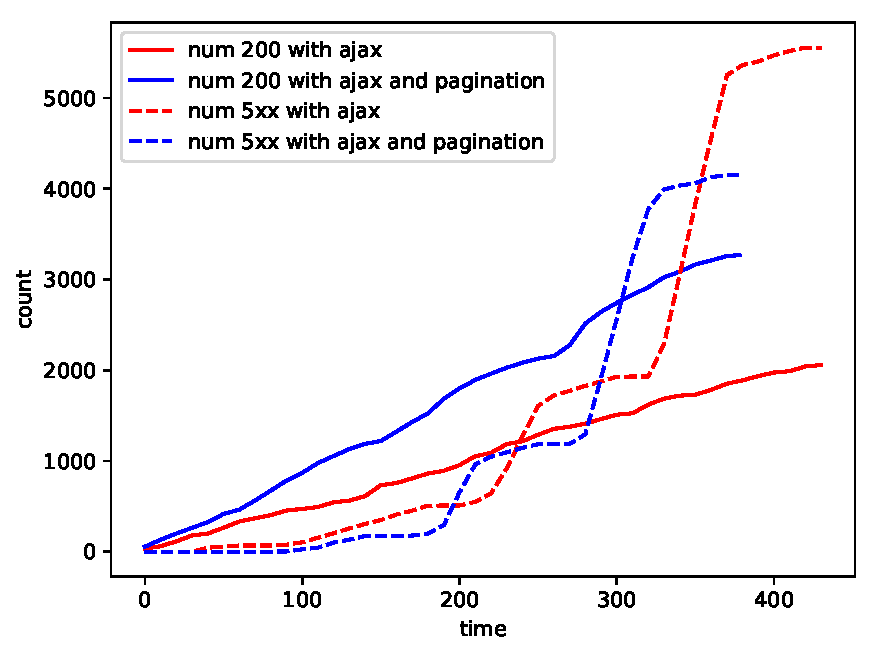
\includegraphics[width=0.46\textwidth]{images/num-code-with-ajax-with-ajax-and-pagination} }}%
    \qquad
    \subfloat[Mean duration of requests.]{{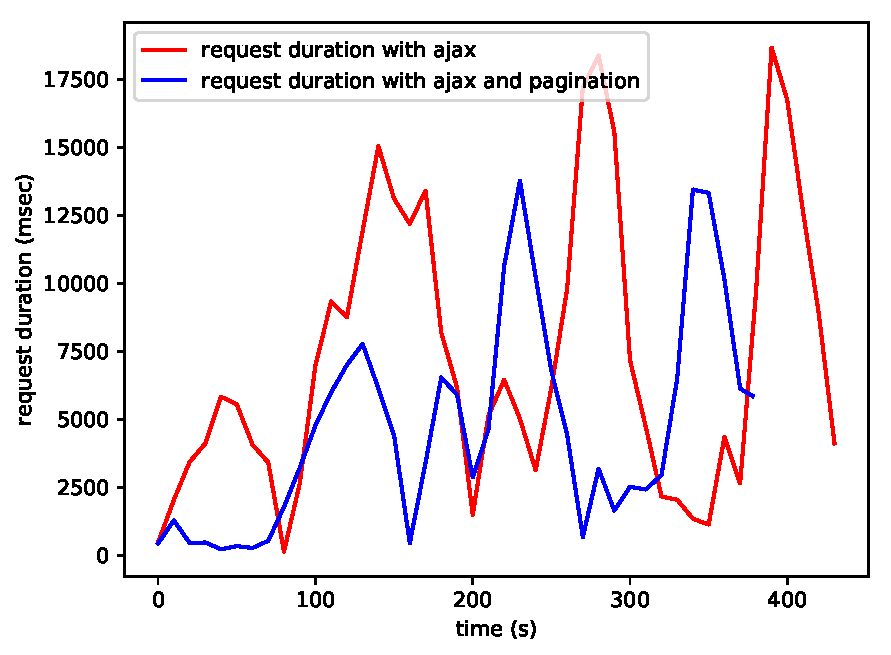
\includegraphics[width=0.46\textwidth]{images/request-duration-with-ajax-with-ajax-and-pagination} }}%
    \caption{Metrics for ajax only and ajax along with pagination.}%
    \label{fig:aap}%
\end{figure}

\section{Optimization: Database Indexing}
The data model of our application was complex. There were multiple different types of relations throughout the database. These relations were queried in one way or another in almost every page of the web app. Therefore we decided to index on the foreign keys of most tables. This resulted in a sharp boost in performance. Figure~\ref{fig:dbindex} shows the mean duration for search transaction (second session of generic workflow as discussed in Section~\ref{sec:generic-workflow}) without and with indexing. It can be observed that indexing made the transaction significantly faster.
\begin{figure}
	\centering
	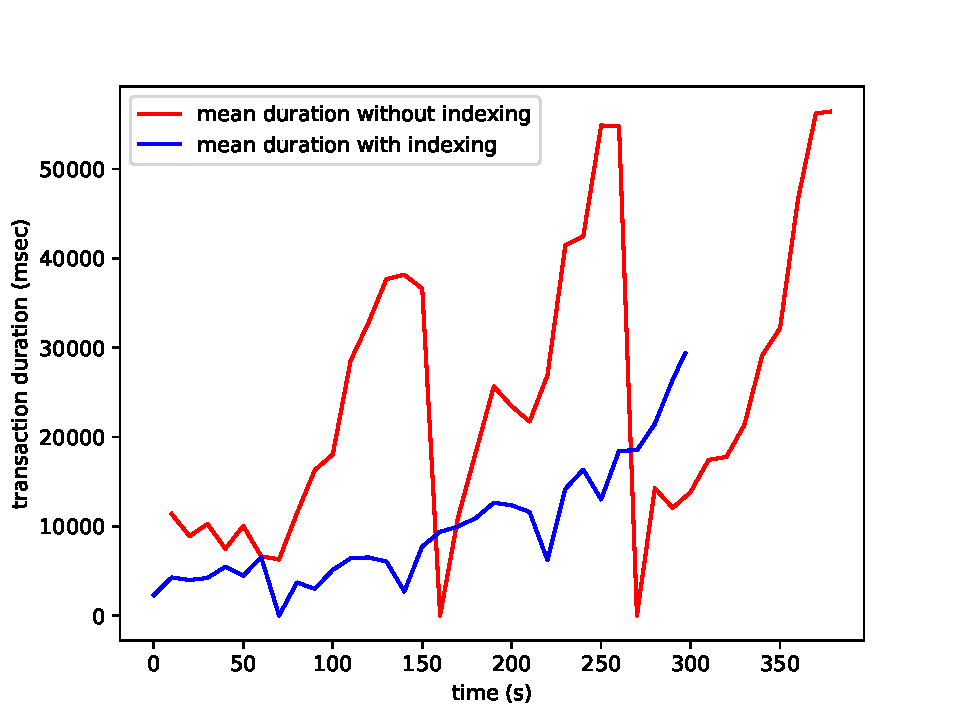
\includegraphics{images/search-transaction-duration-without-indexing-with-indexing}
	\caption{Mean duration for search transaction without and with indexing.}\label{fig:dbindex}
\end{figure}

\section{Optimization: SQL Query}
Careful observation of the Rails log during development revealed that the ``N + 1'' problem of SQL query was prevalent in our application. Specifically, the genres and companies index pages shows the number of games under each genre/company. To retrieve this number, $N$ more queries were triggered in the initial version of the app for $N$ genres/companies apart from the one invoked to get all genres/companies. This situation was later remediated so that instead of ``N + 1'' queries only two queries were invoked. Tsung tests were run on the specific workflow to evaluate the improvement in performance. Figure~\ref{fig:sqlopt} shows the graph of mean duration for the transaction without and with indexing. It is evident from the graph that the discussed SQL optimization greatly improved the response time of the application.
\begin{figure}
	\centering
	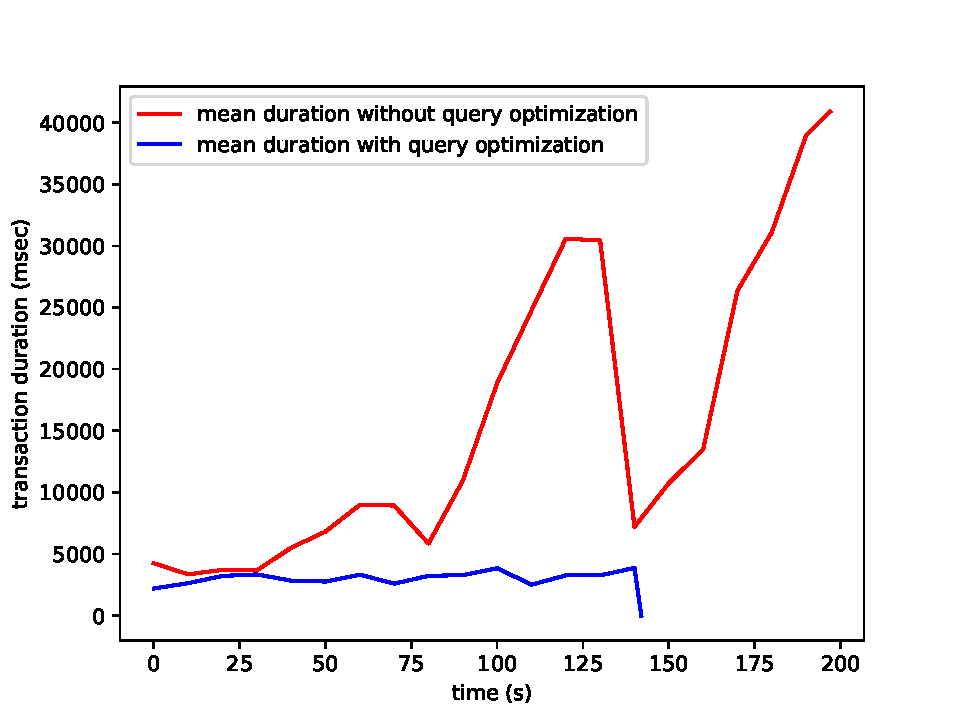
\includegraphics{images/list-pages-transaction-duration-without-query-with-query}
	\caption{Mean duration for index page transaction without and with indexing.}\label{fig:sqlopt}
\end{figure}

\section{Optimization: Caching}
\section{Scaling}
